\documentclass{article}

\usepackage[utf8x]{inputenc}
\usepackage[spanish]{babel}
\usepackage[margin=3cm]{geometry}
\usepackage{amsmath}
\usepackage{amssymb}

\usepackage{graphicx}


\title{Computación Concurrente \\ \Large{Tarea 3}}
\author{
  Diego Goméz Montesinos
  \and
  José Emiliano Cabrera Blancas
  }
\date{25 febrero 2014}
\begin{document}
\maketitle
\begin{enumerate}
\item{
    Recuerden el modelo visto en clase con el que resolvimos la tarea
    $\epsilon$-aggremment para dos procesos. Alice y Bob proponen un valor y
    quieren quedar de acuerdo en un valor que no diste más de $\epsilon$ de lo
    que el otro decidió. Después vimos que necesitaban comunicarse y que para 
    $\epsilon$ más pequeñas se necesitaban más y más rondas de comunicación.
    Recuerden que usamos el modelo de memoria compartida de lectura/escrita por
    capas \textit{full information} (por cada escritura leíamos un nuevo
    arreglo y escribimos todo lo que sabemos cada vez).\\
    Ahora proponemos otros dos modelos de comunicación: el modelo chismoso y el
    modelo discusión civil. El modelo chismoso dice que si Alice y Bob alguno de
    los 2 no escucho al otro entonces tienen otra ronda de comunicación. De lo
    contrario si los dos se escuchan entonces ahi termina la comunicación.
    Podriamos verlo como que se lanzan insultos e indirectas pero no de frente.\\
    El modelo discusión civil dice que mientras Alice y Bob esten escuchando 
    mutuamente la conversación sigue. En el momento que uno ya no escucha al otro
    ahi se termina.
    Sea \textit{M} $≥$ 0 el número de rondas máximo que se pueden comunicar Alice
    y Bob:

    \begin{enumerate}
      \item{Para los 2 modelos dados describe el complejo del protocolo para M. 
        Tienes que dar la tripleta $(I,P_m,\Xi_m)$}\\\\
        
        \textbf{SOLUCIÓN}\\
        Para efectos de este ejercicio la etiqueta A es gris, y B es negro.\\\\
        Considere que para los dos modelos, la entrada $I$ es la siguiente:\\
        \begin{center}
        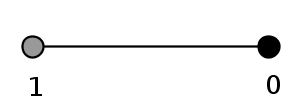
\includegraphics[scale=1.15]{input1a.png}\\
        \scriptsize{Complejo de entrada $I$}\\
        \end{center}
        Recordemos que con el \textit{modelo normal} de memoria compartida por capas,
        en la primera ronda de comunicación, el complejo de entrada anterior se
        mapeaba en el siguiente complejo:
        \begin{center}
        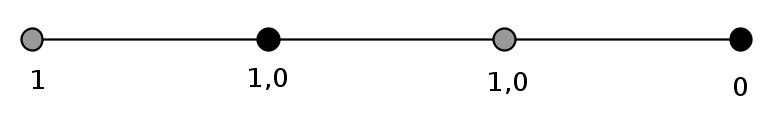
\includegraphics[scale=0.95]{pronda1a.png}\\
        \scriptsize{Complejo en la 1era ronda de comunicación}\\
        \end{center}
        Ahora, primero describiremos el \textit{modelo chismoso}:\\
        Note que en la primera ronda de comunicación de este modelo, el complejo de
        entrada se mapea exactamente al mismo que el complejo anterior (primera ronda del
        modelo normal); ya que tanto es posible que A no vea a B, que B no vea a A y que
        ambos se vean.
        Lo diferente viene a partir de la siguiente ronda de comunicación, ya la arista que
        representa al último caso, donde ambos se ven, ya no tendrá subdivisión por la
        especificación del modelo.\\
        En la siguiente ronda de comunicación, el complejo queda como sigue:
        \begin{center}
        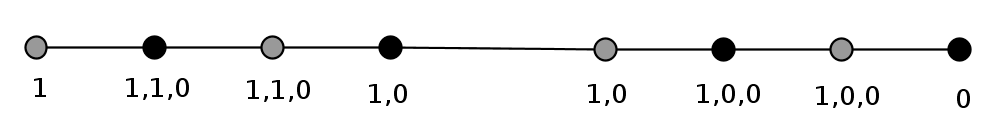
\includegraphics[scale=0.95]{srondachismoso1a.png}\\
        \scriptsize{Complejo en la 2da ronda de comunicación\\en el modelo chismoso}\\
        \end{center}
        Analicemos ahora como cambió el complejo entre las rondas de comunicación y tratemos
        de ver como cambian con las rondas:
        \begin{center}
        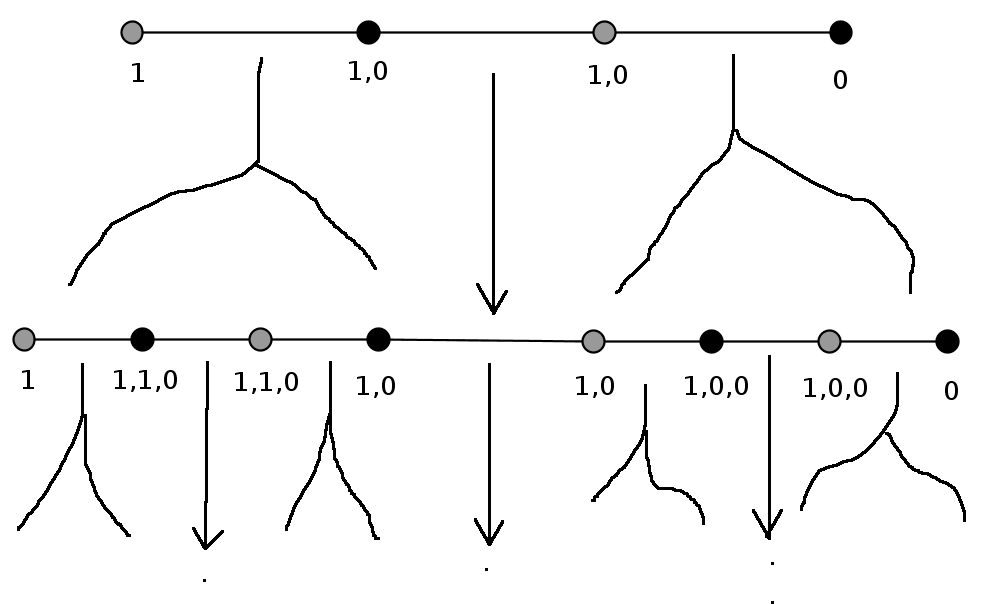
\includegraphics[scale=0.2]{cambiosrondas1a.png}\\
        \scriptsize{Mapeo entre las rondas\\en el modelo chismoso}\\
        \end{center}
        Como se puede ver, en cada ronda de comunicación, hay dos aristas nuevas por cada
        arista que es posible dividirse, y esas a la vez se dividen en dos, y así sucesivamente.
        Además se preserva la arista de enmedio. Esto se parece mucho al crecimiento de un árbol
        binario.
        \begin{center}
        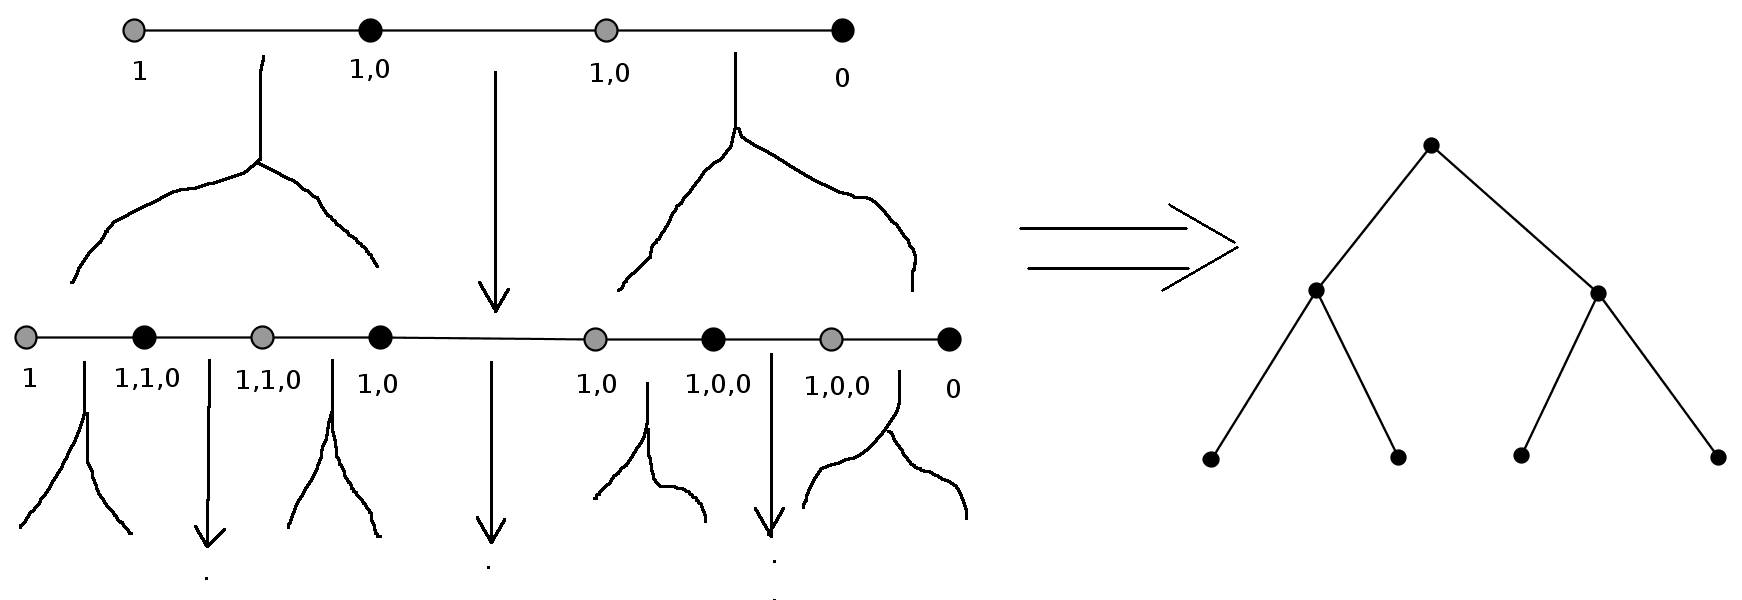
\includegraphics[scale=0.2]{cambioschismosoarbol1a.png}\\
        \scriptsize{Comparación con un árbol binario}\\
        \end{center}
        Con lo anterior tenemos que para \textit{M} $≥$ 0, el número de aristas en la ronda
        \textit{M} es: $2^{M + 1}-1$\\\\
        Ahora veamos el \textit{modelo de discusión civil}:\\
        Note que sucede exactamente lo mismo que en el modelo anterior, solo que en este caso,
        solo habrá una arista que se dividirá (caso en el que los dos se vieron) y las otras dos
        permanecerán iguales (casos en los que uno solo vio a uno).
        El complejo en la siguiente ronda con este modelo es:
        \begin{center}
        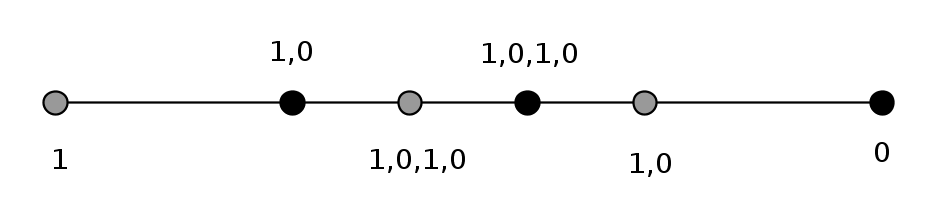
\includegraphics[scale=0.95]{srondacivil1a.png}\\
        \scriptsize{Complejo en la 2da ronda de comunicación\\en el modelo chismoso}\\
        \end{center}
        Como en el modelo anterior, veamos como cambiaron los complejos entre las rondas:
        \begin{center}
        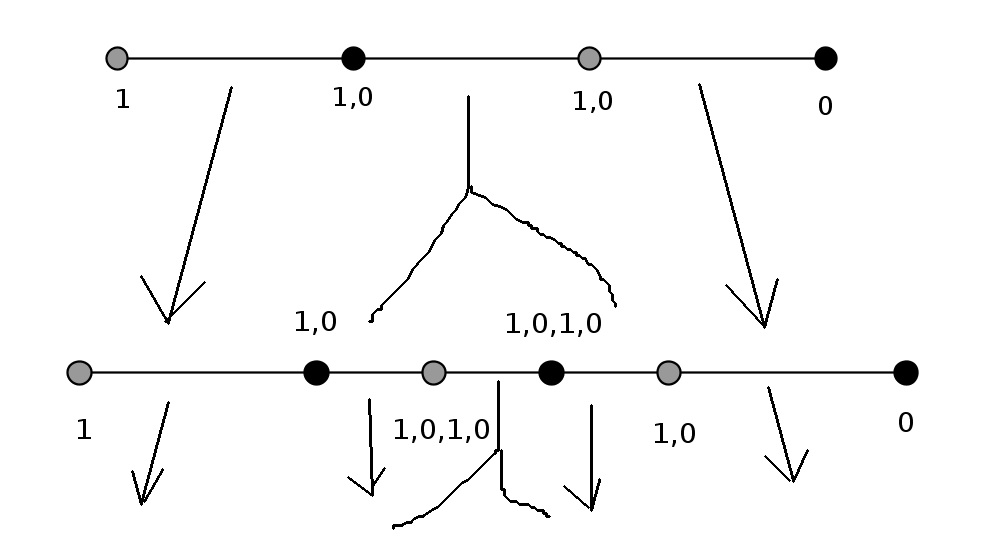
\includegraphics[scale=0.2]{cambiosrondascivil1a.png}\\
        \scriptsize{Mapeo entre las rondas\\en el modelo discusión civil}\\
        \end{center}
        Se puede ver que una arista generará dos nuevas aristas, y conservaremos
        las demás aristas.\\
        Con esto renemos que para \textit{M} $≥$ 0, el número de aristas en la ronda
        \textit{M} es: $2M + 1$\\

      \item{Para los 2 modelos describe cuál es la tarea $\epsilon$-agreement
        óptima para cada \textit{M} $≥$ 0. Nos referimos a óptimo como que cada
        vista del protocolo va a un valor de decisión único. En otras palabras
        encontrar la $\epsilon$ en función de M.}\\\\

        \textbf{SOLUCIÓN}\\
        Con el inciso anterior obtuvimos que en el \textit{modelo chismoso}, para una 
        la ronda \textit{M} el número de aristas es: $2^{M + 1}-1$; y que para el \textit{modelo
        de discusión civil}, para una la ronda \textit{M} el número de aristas es: $2M + 1$.
        Como cada vista del protocolo debe de ir a un valor de decisión único (así se define la tarea
        $\epsilon$-agreement óptima), entonces debe de haber el mismo número de aristas y de vértices
        en ambos casos.\\
        Por lo tanto, el $\epsilon$ para cada modelo son:
        \begin{itemize}
            \item {
                Modelo chismoso: \begin{equation} \epsilon = \frac{1}{2^{M + 1}-1} \end{equation}
            }
            \item {
                Modelo discusión civil: \begin{equation} \epsilon = \frac{1}{2M + 1} \end{equation}
            }
        \end{itemize}
    \end{enumerate}
  }

\item{
    Con el modelo visto en clase define la función de decisión de equidad de género
    $\delta$, que no distingue entre Alice y Bob. Es decir Alice y Bob pueden tener
    ya sea el valor 0 o 1 de entrada. También da la $\delta$ óptima para este caso.
    Aqui debes de tener cuidado de como etiquetas los vértices para que siempre
    se cumpla la $\epsilon$.
  }

\item{
    
    Ahora regresamos al modelo de memoria compartida y modifiquémoslo. Ahora 
    supongamos que tenemos solo una memoria. Es decir ya no tenemos capas y
    sobreescribimos nuestra parte del arreglo cada ronda. También regresamos
    al caso en que Alice propone 0 y Bob 1.
    \begin{enumerate}
      
    \item{Describe el modelo (haz la gráfica) y ve como se ve la gráfica de 
        vistas después de M rondas.
      }

    \item{¿Cuál es la mejor $\epsilon$ que puede resolver en la tarea del 
        $\epsilon$-agreement en M rondas?}
    \end{enumerate}
  }

\end{enumerate}
\end{document}